\chapter{Intelligent tutoring system}
\label{ch:its-implementation}
\glsreset{its}
%(CONTEXT): background for less specialized readers and establish or recalls the importance of the problem
An important aspect of education in the paved path methodology is its efficiency.
Educational activities should not keep the developer from their responsibilities for longer than necessary.
% (NEED): motivates the audience by stating the difference between the desired and actual situation
% ==>shortcomings and goal from my perspective
The efficiency of training on the \gls{scw} platform is lacking.
Because every individual is presented with the same exercises, they often receive training that is too repetitive or too challenging.
%(The TASK) what did I do?
%=> IRT, ITS
I designed an \gls{its} that recommends exercises to each individual at any point in time to provide them with a more appropriate learning pace.
%When evaluating online learning activities, the focus is often wrongfully on completion and dropout rates~\cite{hadi2016driving}. 
%It is perfectly possible, likely even, that learning took place despite the user not completing the course.
%The goal of the \gls{its} should hence be to maximize the opportunity for learning to take place.
% OBJECT
In this chapter, I present the design of the \gls{its} and discuss the used techniques in its implementation in more detail.
%In this chapter we start with an overview of the design of the \gls{its} in Section~\ref{sec:design}.
%In the rest of the chapter we explain the used techniques in more detail.
%First, the collaborative filtering algorithm is detailed in Section~\ref{sec:collab}.
%Next, the psychometric models are discussed in Section~\ref{sec:calib}.

\summarybox{
I designed an \gls{its} that consists of three algorithmic components, one for exercise selection, and one each for estimation of user ability and exercise difficulty.
Exercise selection is achieved through a \gls{cf} algorithm adapted to learning systems.
In such an algorithm, a target user's preference for an exercise is predicted based on the preferences of like-minded users.
Through the use of the psychometric model of \gls{irt}, estimation of both user ability and exercise difficulty can be done at once.
A sanitized data set of over 9 million solved exercises is used to calibrate these algorithms making up the \gls{its}.
}

% SECTIONS
\section{Design}
\label{sec:design}
The design of the \gls{its} shown in Figure~\ref{fig:its-overview} extends the existing functionality of the training platform.
This existing functionality is depicted in orange on the right side of the figure, while components of the \gls{its} are drawn in blue on the left side.
The \gls{its} consists of two loops, it contains three algorithmic components and three types of data collections.

% high level overview of different components of ITS
\begin{figure}
    \centering
    %\input{03-education/plots/its-flowchart-reverse}
    \includegraphics[page=12]{03-education/figures/tikzfigures.pdf}
  \caption[Design of the ITS]{The \Gls{its} consists of two loops. In the main loop, users are served exercises and their answers are processed, before selecting a new exercise. The user history is then regularly used in a secondary loop to estimate both user abilities and exercise difficulties.}
  \label{fig:its-overview} 
\end{figure}

The algorithmic component in the main loop is that of exercise selection.
Selecting the optimal exercise is done through an adapted \gls{cf} algorithm, as will be explained in more detail in Section~\ref{sec:collab}.
In this technique, a recommendation is derived from historical data of like-minded users.
To evaluate this technique, and hence improve it, we need a measure to decide what a good recommendation is.

A useful challenge is a challenge from which the user has learned something and that keeps the user engaged.
That is, a good recommendation system should increase the \textit{ability} of the user, and their \textit{engagement}.
It is easy to keep track of the engagement of the user.
If they continue to play more challenges, that means they stay engaged.
However, in order to determine if a recommendation leads to increased ability, we need to be able to continuously measure the ability of each user.
Another reason to continuously measure the ability of each user is the temporal aspect to learning.
An exercise that is useful to a user at the beginning of their journey is likely no longer an appropriate recommendation once their ability has sufficiently increased.
Hence ability estimation is needed to both determine \textit{if} a challenge was useful to a user, and \textit{when} a challenge was useful.

A very naive way to achieve an ability estimate is simply looking at the accuracy of each user.
A user answering all of the challenges correctly (100\% accuracy), is likely to have a higher ability level than a user answering half of them correctly (50\% accuracy).
If all users completed the exact same challenges, this could give a reasonably accurate representation of their ability level.
In fact, that is exactly the reasoning behind \gls{ctt}~\cite{ctt}.
In a classic test all examinees are given the same (or equivalent) exercises and their accuracy on the test is an indication of their ability level.

However, on the training platform not all users are completing the exact same challenges and this is not desirable, as that would conflict with the goal of individually tailored recommendations.
When users are completing different challenges, accuracy alone is no longer sufficient.
It is possible for one user to maintain a high accuracy doing simple challenges, while another user's accuracy is lower but they are completing difficult challenges.

This is also true for exercises, the difficulty of an exercise can not be accurately estimated through the accuracy of users completing it.
It is possible for one exercise to have a high accuracy because it is mostly attempted by users of a high ability level, while another is often tried by beginners and hence has a lower accuracy.
It is clear that these two remaining algorithmic components in the \gls{its} are tightly coupled.
Both are implemented through the use of psychometric models from the field of \gls{irt} as explained in Section~\ref{sec:calib}.
The calibration techniques of \gls{irt} use the entire user history and take a while to complete.
This is why they are not performed every iteration of the main loop, but at regular intervals in a secondary loop.

\section{Collaborative filtering}
\label{sec:collab}

In this section, I discuss the first algorithmic component of the \gls{its} as depicted in Figure~\ref{fig:its-overview}, the component of exercise selection.

There are many possible factors that determine which exercise to select.
We can easily imagine some factors that are likely to have a big influence, such as the difficulty of the exercise, the vulnerability type, and the programming language.
Research has also shown that individual learning style has an impact on learning performance~\cite{alshammari2015design,schiaffino2008eteacher,graf2006representative,felder1988learning}.
For other factors, it is more difficult to determine how important they are, or if they matter at all.
Some examples are code quality, code legibility, software type, or even just the coding style of the author of the challenge.
There are also likely other factors that we are not yet aware of.

For this reason, it is desirable to create a recommendation system that uses a black box approach.
With this kind of approach it is not necessary to know which factors determine a good recommendation.
There only need to be enough users and challenges, as well as a way to determine if a challenge was useful to a user.

One frequently used technique for recommendation systems is \gls{cf}.
In \gls{cf}, a target user's affinity for items is used to find other users who are most like-minded.
This group's collective affinity for items is then used to predict the target user's affinity for those items.

These types of algorithms are most easily understood through a visual representation. 
In Figure~\ref{fig:cf}, a simple example of a \gls{cf} algorithm is illustrated.
In this figure, the recorded affinity of users $i$ $(i = 0,\dots,5)$ for movies $j$ $(j = A,\dots,J)$ is depicted in a two dimensional grid.
A green check mark in the grid means that the user enjoyed the movie, a red cross means they did not.
There are also many empty spaces as not all users have watched all movies.
In order to predict the affinity of a target user $i = 0$ for a target movie $j = B$, the \gls{cf} algorithm starts by finding the users who are most like-minded, the users who have the most similar recorded affinity.
For each user, the algorithm determines for how many movies they have the same affinity as the target user.
In Figure~\ref{fig:cf}, the affinity of the target user is marked with an orange background, affinity of other users that is the same as the target user is marked with a green background.
In the example, user $i = 1$ enjoyed movies $j \in \{A,C\}$.
But their affinity for movie $C$ is the only affinity they have in common with the target user.
Users $i \in \{2,3,5\}$ each have the same affinity as the target user for two of the movies. 
In this example, they make up the group of people that are most like-minded to the target user.
To predict if the target user would enjoy the target movie $j = B$, the algorithm now uses this group's affinity for the target movie, marked in a blue background in Figure~\ref{fig:cf}.
Two of the most like-minded users enjoyed the movie and one of them did not.
Since the majority of like-minded users enjoy the target movie, the algorithm predicts the target user might enjoy it as well.

\begin{figure}
    \centering
    %\input{03-education/plots/collaborative-filtering}
    \includegraphics[page=7,width=\textwidth]{03-education/figures/tikzfigures.pdf}
    \caption[Collaborative filtering algorithm]{Visual representation of the steps to determine if the target movie $j=B$ is a good recommendation for the target user $i=0$. 
    The \gls{cf} algorithm first finds all users who have similar preferences for movies as the target user (marked in green). 
    The users who have the most similar preferences are used in a majority vote. 
    In the example users 2, 3, and 5 each had the same preference as the target user for two different movies.
    The majority of these users enjoyed the target movie (marked in blue), so the algorithm concludes that the target is a good recommendation.}
    \label{fig:cf}
\end{figure}

\subsection{Adapted to learning systems}
\label{sec:adapted-cf}
Some adjustments are needed to apply \gls{cf} to a learning system.
In a learning system, a good recommendation is one that allows meaningful learning to take place and at the same time keeps the user engaged.
A good recommendation is hence based on the \textit{utility} of a user for an item, rather than their affinity.
If the users who are most like-minded increased their ability level through playing this challenge, it is likely a good recommendation.

As mentioned before, learning also has a more apparent temporal aspect to it.
An exercise that is useful to a user at the start is no longer an appropriate recommendation once their ability has increased sufficiently.
It could hence be beneficial to keep track of the ability level around which a recommendation can be deemed appropriate.
The \gls{cf} algorithm can then only consider users to be like-minded, if they experienced the same utility as the target user within a certain ability range.
Users who experienced the same utility for an item but at a sufficiently dissimilar ability level will not be considered like-minded users.

Figure~\ref{fig:3d-cf} illustrates how this adaptation could be achieved on the example algorithm from before.
In this figure, the recorded utility that the users $i$ $(i = 0,\dots,5)$ experienced from challenges $j$ $(j = A,\dots,J)$ is depicted in a two dimensional grid for three sufficiently distinct ability levels $\bm\theta$.
A green check mark means that this challenge was useful to the user around that ability level.
A red cross means it was not useful, and the user either did not learn anything, or the challenge caused the user to disengage from the training.
How the utility of a challenge is determined will be explained in Section~\ref{sec:utility}.
To predict the utility of the target challenge $j = B$ to the target user $i = 0$, the adapted \gls{cf} algorithm looks for the most like-minded users, the users who experienced the most similar utility.

However, only if the same utility was experienced around the same ability level does it count towards like-mindedness.
In Figure~\ref{fig:3d-cf}, utility that was experienced by the target user for challenges is marked with an orange background.
Similar utility that was experienced around the same ability level is marked with a green background.
At the lowest ability level, user $i = 2$ experienced the same utility as the target user for four challenges.
User $i = 1$, just like the target user, experienced challenge $j = C$ as useful.
However, the challenge was useful to user $i = 1$ at the lowest ability level, while the target user found this challenge useful when their ability level was sufficiently higher.
Similar utility like this that was experienced around a different ability level is marked with a red background in the figure.
This utility does not count towards like-mindedness.
Using this metric for like-mindedness, we find that users $i \in \{2,3,5\}$ each experienced the same utility around the same ability level as the target user for four different challenges.
They make up the group of users who are most like-minded to the target user.

Beyond this adaptation, the same steps are used to decide the final recommendation.
The majority of like-minded users experienced the target challenge as useful around the targeted ability level, marked with a blue background.
The algorithm concludes that the target challenge is a good recommendation for the target user.

\begin{figure}
    \centering
    %\input{03-education/plots/3d-collaborative-filtering}
    \includegraphics[width=\textwidth,page=3]{03-education/figures/tikzfigures.pdf}
    \caption[Adapted collaborative filtering algorithm]{Visual representation of the steps to determine if the target challenge $j=B$ is a good recommendation for the target user $i=0$. 
    The collaborative filtering algorithm first finds all users who experienced similar utility from challenges as the target user around the same ability level $\bm\theta$ (marked in green). 
    Similar utility at a different ability level is disregarded (marked in red).
    The users who experienced the most similar utility are used in a majority vote. 
    In the example, users 2, 3, and 5 each experienced the same utility as the target user for four different challenges.
    The majority of these users experienced the target challenge as useful (marked in blue), so the algorithm concludes that the target is a good recommendation.}
    \label{fig:3d-cf}
\end{figure}

\subsection{Types of collaborative filtering}
In the examples until now, the affinity (or utility) of a user for an item was considered binary, the user either liked it, or they did not.
In reality, often a more complex scale is used.
For example, Netflix movie recommendations use a rating scale between 1 and 5.
In this context, the affinity of a user $u$ for an item $i$ is often called the rating $r_{ui}$.
The goal of a \gls{cf} algorithm is then to make a prediction for this rating $\hat{r}_{ui}$.
\Gls{cf} algorithms can be split into two broad categories, memory-based and model-based algorithms, based on how they set out to achieve this goal~\cite{li2021novel,sharma2017collaborative,yu2004probabilistic,breese2013empirical,su2009survey}.

\subsubsection{Memory-based}
Memory-based \gls{cf} algorithms directly use observed ratings to compute predictions.
Generally, these algorithms mark a subset of users as neighbours to the target user by calculating the similarity between users~\cite{li2021novel,Hug2020}.
They then use the neighbour's ratings to predict the rating of the target user~\cite{su2009survey,Hug2020,Koren2010,Ricci2010}.

Memory-based \gls{cf} algorithms are frequently used in recommender systems and even commercial systems such as the Amazon webstore~\cite{sharma2017collaborative,yu2004probabilistic}.
The main advantages of memory-based collaborative filtering algorithms are that they are easy to implement, and that new data can be added easily and incrementally.
Their biggest shortcoming is a decreased performance for sparse data, when it is difficult to find sufficient neighbours.
They also can not make recommendations for new users or items as there is no data to do similarity computations with.
In the \gls{its} however, we already need sufficient data to compute the difficulty and ability estimates.
In a learning system, the need for an initial calibration phase can not be avoided, so this shortcoming does not impact the design of the \gls{its}.

Five different memory-based \gls{cf} algorithms are considered in this work. 
They will be described in more detail in the experiments in Section~\ref{sec:eval-cf}.
Four of these algorithms are \gls{knn} algorithms, they first determine the k nearest neighbours and then use the ratings of these neighbours to compute a prediction.
Because these algorithms use an explicit definition of similarity between users, they can be easily adapted to learning systems by changing this definition to take into account the ability of the users.
The remaining memory-based algorithm uses the ratings of all users to make a prediction, adapting it to learning systems will be harder, but can still be achieved by processing the data, as will be explained in the description of the experiments.

\subsubsection{Model-based}
Model-based \gls{cf} algorithms use statistical and machine learning methods to construct a model, and use this model to make predictions~\cite{sharma2017collaborative, li2021novel,sarwar2002recommender,heckerman2000dependency}.
These models often use techniques to reduce the dimensions of the matrix of user-item ratings.
This reduces the scalability and sparsity problems that are experienced by memory-based algorithms~\cite{sarwar2002recommender,moreno2016web}.
Model-based algorithms are often more accurate, but the construction of the model is often slow and expensive, and they have to be re-built regularly, every time new data is being added incrementally.

Algorithms using clustering techniques are simple examples of model-based algorithms~\cite{su2009survey,breese2013empirical,sarwar2002recommender,o1999clustering}.
Users or items are assigned to one or more clusters so that the matrix of user-item ratings becomes a smaller, denser matrix of clusters.
It is then possible to use statistics from these clusters to make predictions, for example, by taking the average rating of a cluster.
In the experiments of this work, one clustering algorithm is evaluated.

Thanks to their accuracy and scalability, model-based algorithms based on matrix factorization have gained a lot in popularity~\cite{Ricci2010}.
These algorithms use the technique of \gls{svd} to make a low rank approximation of the original ratings matrix~\cite{george2005scalable, Ricci2010, Hug2020}.
\Gls{svd} is a well-established technique in linear algebra and machine learning to identify latent semantic factors.
Applying it in the \gls{cf} domain raises a few difficulties due to the sparsity of the rating matrix, which increases the risk of overfitting.

In the experiments of this work, I evaluated \gls{pmf}~\cite{mnih2008probabilistic}, \gls{nnmf}~\cite{wang2012nonnegative,hoyer2004non}, \gls{svd}~\cite{sarwar2000application,polat2005svd,Ricci2010}, and \gls{svd}++~\cite{koren2008factorization,Ricci2010}.
All of these algorithms are explained in more detail in Section~\ref{sec:eval-cf}.

\subsection{Alternative approaches}
\label{sec:cf-alternatives}
Many existing alternatives either do not take into account the ability level of the users to make recommendations, or they only take into account the ability level~\cite{chen2005personalized}.

\subsubsection{Adaptive learning systems}
Many computerized learning systems already exist, both in commercial offerings and in research literature.
Older systems do not consider individual learners needs, but make decisions based on pre-planned instructions for the field of study.
As a result, these systems do not provide individual attention to students as a natural (human) teacher would~\cite{mahdi2016intelligent}.
This inspired the rise of more advanced learning systems that consider both the field and the learner to provide flexibility in the presentation of the educational material.
Some such systems have been built to teach computer science concepts, such as debugging~\cite{carter2013tutoring}, cryptographic algorithms~\cite{abuel2018intelligent,mahdi2016intelligent}, programming in C++~\cite{abu2009evaluating}, or \gls{sql}~\cite{mitrovic2003intelligent}.

These systems have varying degrees of intelligence and adaptiveness.
In commercial offerings, such as Pluralsight Iris\footnote{\url{https://www.pluralsight.com/product/iris}}, adaptive learning often refers to an initial calibration phase to determine the initial ability level of a user.
In other systems, students are allowed to advance to more difficult levels when a sufficiently high accuracy is achieved on exercises in the current level~\cite{abu2009evaluating,mahdi2016intelligent}.
Even more advanced systems provide adaptive feedback to the users, based on which mistakes have been made in the exercises~\cite{carter2013tutoring,abuel2018intelligent}.
Finally, the most advanced systems are able to adapt the difficulty of the exercises more dynamically.
Duolingo for example, adapts the difficulty of the of last few exercises in a lesson based on the performance of the student on the previous exercises\footnote{\url{https://blog.duolingo.com/}}.

All of these system focus on offering exercises of the appropriate difficulty level, and some also take into account classifications of learning styles~\cite{alshammari2015design,felder1988learning}.
The goal of the \gls{its}, however, is to also pay attention to other potential factors such as the coding style, presentation form, application type, and so on.
The discussed systems could potentially be adapted to take into account several of these factors.

\subsubsection{Serious games}
Several serious games exist to for topics related to cybersecurity and social engineering.
They usually focus on increasing the awareness of software users of different ages and are not used to train software developers~\cite{giannakas2015cyberaware,jin2018evaluation,beckers2016serious,yasin2018design}.

Research in this field mostly focuses on the effect of gamification, and usually adds game elements to static learning content.
They usually do not adapt to the users beyond opening up new content after the completion of preceding exercises.
While gamification leads to increased engagement, this is not the focus of my research as I believe the \gls{scw} platform already has some decent gamification features.

\subsubsection{Content-based recommendation systems}
Another type of recommendation system that is related to \gls{cf} algorithms, is content-based recommenders.
These systems analyze item descriptions to identify items that are of particular interest to a user~\cite{pazzani2007content}.
To do this, they represent both items and users as a vector of characteristics, similar to vectors in the latent space used by model-based \gls{cf} algorithms.
However, in contrast with these \gls{cf} algorithms, the vectors are not computed in a latent space by the algorithm.

Item characteristics are often already available in the system, or they can be detected through natural language processing.
They are often easier to interpret than the dimensions of the latent space in model-based algorithms.
On the \gls{scw} platform, the framework, language, vulnerability type, and author are examples of characteristics that are readily available.

In order to make a recommendation for a user, items are selected that have similar characteristics to previously liked items by this user.
Several algorithms can be used to achieve this, among which nearest neighbour methods and decision trees~\cite{pazzani2007content}.
In contrast with item-based collaborative filtering, these algorithms compute the similarity between items based on the characteristics of the items themselves.
While in \gls{cf} algorithm the similarity between items is based on the similarity of ratings these items receive by users.
This is likely not a good approach for learning systems, where diverse content should be recommended, covering, for example, multiple vulnerability types.

\subsubsection{Knowledge-based recommendation systems}
Systems that make use of the organisation of learning material are called knowledge-based, or semantics-based recommendation systems.
They create a structured knowledge graph or ontology to organise the learning material.

Existing ontologies in software security attempt to organize different security concepts in a broader knowledge graph of computer science.
For example, they classify \gls{sql} injection as a type of injection attack, \gls{sql} security as a type of data integrity, and a \gls{dos} attack is linked the availability of the product~\cite{kang2013security, jia2018practical}.
While this information can be useful to a developer learning about different security concepts, it can not be used to organise the learning material on the \gls{scw} training platform.

Many vulnerability types require a broad knowledge of varying aspects of software development, such as the operating system, communication protocols, language and framework specifics, software architecture, and more.
On the \gls{scw} platform, however, we assume the users have sufficient knowledge of these domains, and require education in software security only.
With this assumption, I do not see a need to create a knowledge graph for software vulnerabilities.
It is my belief that most vulnerabilities are unrelated to each other, in the sense that it is possible to understand and master each of them without the need to learn about the other.
Current education efforts often focus on the \gls{owasp} top 10, in which vulnerabilities are ranked mostly based on their prevalence in practice.
This is strong evidence for the fact that the order they are being taught to developers is not of big importance.

\subsubsection{Computerized Adaptive Tests}
\Glspl{cat} are computer-based tests that adapt to the ability of the examinee. 
They continuously estimate the ability level and serve the next test item based on the current estimate.
While there are techniques from \glspl{cat} that are useful to us, as will be explained in Section~\ref{sec:calib}, the item selection is not appropriate for use in the \gls{its}.

This is because the goal of a test is to estimate the ability of an examinee. \Glspl{cat} are able to maintain a higher precision of ability estimation while being about 50\% shorter compared to \glspl{fit}~\cite{weiss1984application}.
To estimate the examinee's ability in such an efficient way, \glspl{cat} select the next item in a test based on which one provides the most information about the examinee. 
These are the items for which the probability of a correct answer is around 50\%~\cite{magis2017computerized, ling2017computerized}.

This goal is of course different from that of the \gls{its} which is to motivate and engage the users. 
In fact, the opposite is even true, tests are inherently not very motivating.
Certainly that is the case for \glspl{cat}, where the examinee is only expected to correctly answer half of the test questions.
Research has shown that engagement can be improved, and anxiety reduced, by choosing items for which the probability of a correct answer is higher (e.g. 70\%)~\cite{ling2017computerized}. 
Still, the item selection algorithm in \glspl{cat} only takes into account the difficulty of the items. 
As discussed before, we want the \gls{its} to possibly take into account other aspects of the exercises, such as coding style, author, or application type.
\section{Difficulty estimation and ability estimation}
\label{sec:calib}
% These two are not always independent:
% Getting difficult challenges correct should have more impact than getting easy challenges correct
% Skilled users answering an exercise correct should have a different impact than unskilled users answering an exercise incorrect

%Difficulty is based on the amount of options this challenge has in the identify stage. Completely irrelevant for the other stages. And not related at all to the code quality, vulnerability type, code complexity etc
%Mention exact algorithm here!

%A score is rewarded to players after completion
%Based on performance and difficulty of the challenge
%the high score also does not accurately represent skill level

% Ability level is needed for two tasks in the system:
% 1. We need accurate absolute ability estimation for temporal aspect of a recommendation
% 2. and fast relative ability estimation for deciding if a challenge is useful or not
In the previous section, I discussed the component of exercise selection, the first algorithmic component of the \gls{its} as shown in Figure~\ref{fig:its-overview}.
This algorithmic component is implemented through the use of a \gls{cf} algorithm.
In order to use this algorithm effectively in a learning system, we need an accurate ability measure.
This ability measure is necessary to both determine \textit{if} a challenge was useful, and \textit{when} a challenge was useful.
In this section, I discuss ability estimation, together with difficulty estimation, the two remaining algorithmic components of the \gls{its}.
I explain how both can be implemented simultaneously by using \gls{irt}, a technique borrowed from the field of psychometrics.
This field of study focuses on the objective measurement of skills, knowledge, and abilities, often with the goal to create better computerized tests.

The goal of a test is to estimate the ability of an examinee.
With \glspl{cat}, this can be done with higher precision while using less exercises than classic \glspl{fit}.
To achieve this, \glspl{cat} continuously adapt the exercises to the estimated ability level of the examinee.
An overview of the steps taken by a \gls{cat} is shown in Algorithm \ref{al:test}. 

\begin{algorithm}[H]
\SetAlgoLined
\SetKwInOut{Input}{\textcolor{scw-red}{input}}
\SetKwInOut{Output}{output}
\Input{calibrated item bank $I$}
\Output{ability level $\bm{\theta}$}
Set $\bm{\theta}$ to entry level\;
\While{termination criterion not met}{
  Select optimal item $i$ from $I$ based on $\bm{\theta}$\;
  Present $i$ to examinee\;
  Update $\bm{\theta}$ based on all prior answers\;
 }
\caption{\label{al:test}A computerized adaptive test}
\end{algorithm}

Some key components are needed to create such a test: calibrated test items, a termination criterion, a starting point or entry level, an item selection algorithm, and an ability estimation algorithm.
We can easily see parallels between a \gls{cat} and the \gls{its}. 
First, test items in a \gls{cat} need to be calibrated, similarly to the exercises in the \gls{its}. 
Secondly, it is necessary in both systems to continuously estimate the ability of the users. 
Finally, there is also a selection algorithm that determines which item the user is shown next. 
However, the item selection algorithm in a \gls{cat} is designed with a different goal in mind, as discussed in Section~\ref{sec:cf-alternatives}. 

\Glspl{cat} frequently use the psychometric model \gls{irt}.
This model not only allows calibration of both users and items, but because they are placed on the same scale, the results can easily be used for item selection as well.
Although it will not be used for exercise selection in the \gls{its}, the model is certainly useful for accurately estimating exercise difficulty and user ability. 

\subsection{Item response theory}
\label{sec:irt-intro}
\Gls{irt} is a model for measuring psychological \textit{latent traits}, i.e. unobservable characteristics such as ability or competence level. 
The model estimates these latent traits by means of \textit{manifest} (observable) variables and statistical psychometric models.
This is done based on the mathematical relationship between the latent traits and the manifest variables. 
A user with a higher ability level (latent trait) is more likely to answer more questions, and more difficult questions, correctly (manifest variables). 
This relationship can be written down as a mathematical function, called the \gls{irf}. It describes the possibility of observing each possible answer as a function of person ability levels and exercise parameters.

\begin{equation}
    \label{eq:irf}
    P_{jk}(\bm{\theta}_i,\bm{p}_j) = Pr(X_{ij} = k | \bm{\theta}_i,\bm{p}_j) = f(k,\bm{\theta}_i,\bm{p}_j)
\end{equation}

In Equation \ref{eq:irf} the ability level of a person $i$ $(i = 1,\dots,I)$ is represented by a multivariate vector of latent traits $\bm{\theta}_i$. $\bm{p}_j$ is the set of parameters of exercise $j$ $(j = 1,\dots,J)$. $X_{ij}$ is the answer of person $i$ for exercise $j$, with $k$ representing one possible answer. 
For dichotomously scored exercises (e.g. true/false) $k \in \{0,1\}$, for polytomously scored exercises (e.g. multiple choice) $k \in \{0,\dots,K_j\}$. 
There are many mathematical functions that can be used to describe the \gls{irf}, each resulting in a different \gls{irt} model.
The most common, and the one used in the \gls{its}, is called the Rasch model, and will be explained in the next Section.

The Rasch model is a dichotomous model.
It is necessary to use a dichotomous model in the \gls{its} because some important data is missing to use polytomous models effectively.
Polytomous models are most effective when the number of possible options for the multiple choice question is limited to three or four. 
The incorrect options need to be deliberate and able to mislead a person with a lower ability level. 

On the \gls{scw} training platform, this is not the case as will be explained in Section~\ref{sec:data}.
Because of this lack of useful polytomous information, I decided to use the dichotomous Rasch model.
For dichotomous models, there are only two outcomes, $k \in \{0,1\}$, representing correct and incorrect.
That means the \gls{irf} in Equation \ref{eq:irf} can be reduced to

\begin{subequations}
\label{eq:irf-dicho}
\begin{align}
        P_{j1}(\bm{\theta}_i,\bm{p}_j) = Pr(X_{ij} = 1 | \bm{\theta}_i,\bm{p}_j) &= P_{j}(\bm{\theta}_i,\bm{p}_j) ,         \label{eq:irf-dicho1} \\
        P_{j0}(\bm{\theta}_i,\bm{p}_j) = Pr(X_{ij} = 0 | \bm{\theta}_i,\bm{p}_j)
        &= 1 - P_{j}(\bm{\theta}_i,\bm{p}_j)
        = Q_{j}(\bm{\theta}_i,\bm{p}_j) ,         \label{eq:irf-dicho2}
\end{align}
\end{subequations}

such that $P_{j}$ represents the probability of a correct response for exercise $j$, and $Q_j$ the probability of an incorrect response.

\subsection{Rasch model}
\label{sec:rasch}
Several mathematical functions can be used to characterize the \glspl{irf} in Equations \ref{eq:irf-dicho1} and \ref{eq:irf-dicho2}.
The most commonly used are logistic distribution functions, resulting in the so-called Rasch model~\cite{rasch1960probabilistic}.

%\todo[inline]{Add advantages of Rash model here or is this out of scope of the work?}
%Rasch modeling allows for generalizability across samples and items, takes into account that response options may not be psychologically equally spaced, allows for testing of unidimensionality, produces an ordered set of items, and identifies poorly functioning items as well as unexpected responses. Each of these characteristics becomes a potential advantage to be exploited.

%Rasch modeling is new to the field of counseling psychology, and only time will determine whether the advantages are sufficient to warrant use. However, several of the advantages appear promising. For example, the ability to identify unexpected results has research and clinical applications. In classical test models, outliers are identified by extreme scores, but we take scores in the middle ranges to be acceptable, as long as the instrument has generally been shown to be reliable. Rasch modeling would identify a research participant who had responded randomly to the instrument (therefore scoring near the mean) or idiosyncratically to a few items. Similarly, clinicians using scales designed on the basis of Rasch modeling could identify clients who responded unexpectedly (and without resort to separate scales, such as is the case with the Minnesota Multiphasic Personality Inventory).

In its simplest form the Rasch model takes only one parameter $\bm{p}_j = b_j$ representing the difficulty of the exercise. 
The \gls{irf} using a one-parameter logistic distribution function is shown in Equation~\ref{eq:1pl}.

\begin{equation}
    \label{eq:1pl}
    P_{j}(\bm{\theta}_i,\bm{p}_j) =
    Pr(X_{ij} = 1 | \bm{\theta}_i,b_j) =
    \frac{\exp(\theta_i - b_j)}{1 + \exp(\theta_i - b_j)}
\end{equation}

The resulting model is called the \gls{1pl}. 
In Figure~\ref{fig:1pl} the \gls{irf} of the \gls{1pl} model is plotted for three exercises with various values for the difficulty parameter.
In this model, for a fixed ability level $\bm\theta$, the probability of a correct answer $P_j$ is lower for exercises with a larger difficulty $b_j$.
The probability takes the value of 0.5 when the ability level of the user exactly matches the difficulty of the item.
This is a result of placing the user abilities and the item difficulties on the same scale.

\begin{figure}
    \centering
    %\input{03-education/plots/1pl}
    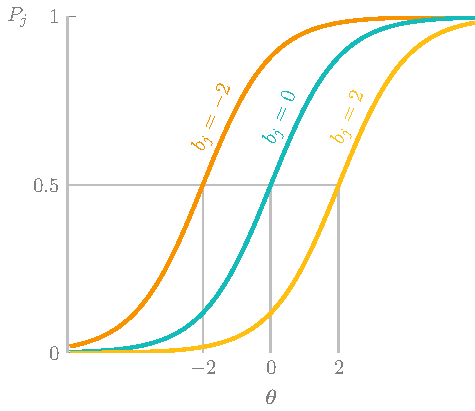
\includegraphics[page=1]{03-education/figures/tikzfigures.pdf}
    \caption[Item response functions of the 1PL model]{Three \glspl{irf} in the \gls{1pl} model, with different difficulty parameters $b_j$. The difficulty parameter represents the difficulty of the exercise. 
    For a fixed ability level, e.g. $\bm\theta = 0$, a higher difficulty means a lower probability $P_j$ of getting a correct answer.
    The probability of a correct answer is 50\% when $b_j = \bm\theta$.}
    \label{fig:1pl}
\end{figure}

There are more characteristics to an exercise than its difficulty. 
One characteristic that is useful to help estimate the ability of users is the discriminative ability of the exercise.
This characteristic represents how good an exercise is at differentiating between users of varying ability levels.
An extension to the \gls{1pl} model exists that includes this parameter, resulting in the \gls{2pl}. 
This second parameter $a_j$ of an item is a multiplicative parameter, as shown in the \gls{irf} in Equation~\ref{eq:2pl}.

\begin{equation}
    \label{eq:2pl}
    P_{j}(\bm{\theta}_i,\bm{p}_j) =
    Pr(X_{ij} = 1 | \bm{\theta}_i,a_j,b_j) =
    \frac{\exp\big[a_j(\theta_i - b_j)\big]}{1 + \exp\big[a_j(\theta_i - b_j)\big]}
\end{equation}

In Figure~\ref{fig:2pl} the \glspl{irf} are plotted for three exercises with the same difficulty $b_j = 0$ but various discriminative abilities. 
For all three \glspl{irf} the probability of a correct answer is still 0.5 for users with an ability level equal to the exercise difficulty.
However, the second parameter influences the steepness of the curve.
For larger discrimination parameters such as $a_3 = 4$, a smaller increase in ability $\bm\theta$ around the exercise difficulty level $b_j = 0$ leads to a more notable increase in probability of a correct answer $P_j$.
Such an exercise discriminates better between low and high ability users.
On the other hand, exercises with lower discrimination values, like $a_1 = 0.25$ result in flatter \glspl{irf} and do not allow as easily for such discrimination.

\begin{figure}
    \centering
    %\input{03-education/plots/2pl}
    \includegraphics[page=2]{03-education/figures/tikzfigures.pdf}
    \caption[Item response functions of the 2PL model]{Three \glspl{irf} in the \gls{2pl} model, with equal difficulty parameter $b_j$ but different discrimination parameters $a_j$. The discrimination parameter represents how well an exercise can differentiate between users of different ability levels $\bm\theta$. A higher value means a steeper increase in probability of a correct answer $P_j$ around the difficulty level $\bm\theta = b_j$.}
    \label{fig:2pl}
\end{figure}

%Figure~\ref{fig:its-architecture} shows the completed architecture of the \gls{its}, obtained by replacing the algorithmic components with the techniques explained in this section.
%
%\begin{figure}
%    \centering
%    \input{03-education/plots/its-filled}
%  \caption{todo}
%  \label{fig:its-architecture} 
%\end{figure}

\subsubsection{Model calibration}
Both the \gls{1pl} and \gls{2pl} models hold parameters of two types: item parameters $\bm{p}_j$ and person parameters $\bm{\theta}_i$. 
With enough data, both sets of parameters can be accurately estimated.
First, the item parameters are estimated independently of the ability levels, this is called the \textit{model calibration}. 
Next, the ability levels are estimated while keeping the item parameters fixed.

\Gls{irt} offers several model calibration techniques, mostly designed for item banks with several dozens of items.
The larger size of the item bank of \gls{scw} will cause longer execution times and more difficult convergence to stable estimates.
I solve this problem by splitting the item bank to several smaller item banks, for example one for each framework on the platform.
The resulting consequences are discussed in Chapter~\ref{ch:its-experiments}.

The calibration of the model consists of tuning the model parameters to maximize the likelihood of the observed data.
More formally, model calibration is maximizing the likelihood of the model $L(\bm\theta,\bm{p})$ with respect to all item parameters $\bm{p} = (\bm{p}_1,\dots,\bm{p}_J)$.
Because this likelihood is also dependent on all person parameters $\bm\theta = (\theta_1,\dots,\theta_I)$, direct maximization is not possible.
There are several possible techniques that can be used to overcome this.
The most well-known are \gls{jml}, \gls{cml}, and \gls{mml}~\cite{magis2017computerized}.

The \gls{jml} algorithm iteratively maximizes the full likelihood with respect to both person and item parameters until convergence is reached.

\Gls{cml} relies on properties specific to the Rasch model to replace unknown ability levels with known sufficient statistics which then allows for the estimation of the item parameters without requiring the estimation of the person parameters.

\Gls{mml} is formulated under the assumption that the ability is a random parameter.
In contrast to the \gls{cml}, it can be used for other \gls{irt} models besides the Rasch model~\cite{bartolucci2010point}.
It does not replace the person parameters by sufficient statistics, but aims to integrate out the person parameters from the maximization process~\cite{bartolucci2010point,magis2017computerized}.
A prior distribution for the ability parameters $f(\bm{\theta})$ is used to compute the marginal likelihood (or the expectation) of a response pattern as shown in Equation~\ref{eq:integrate-out}.

\begin{equation}
    \label{eq:integrate-out}
    P_{j}(\bm{p}_j) = \int_{\mathbb{R}} P_{j}(\bm{\theta}_i,\bm{p}_j) f(\bm{\theta}_i) d\bm{\theta}_i
\end{equation}

The prior distributions are often chosen as normal distributions.
The item parameters can then be estimated by maximizing the full likelihood, calculated as the product of all marginal pattern likelihoods.
Computing these marginal response pattern distributions was conceptually complex until efficient \gls{em} algorithms were implemented~\cite{magis2017computerized}.

In this work, I used the \gls{mml} approach as it has many advantages, such as its applicability to many types of \gls{irt} models, its ability to compare the fit of different models, and its ability to handle perfect response patterns (all correct or all incorrect answers).

\subsubsection{Ability estimation}
Once the item parameters are calibrated, they are set as fixed.
Estimating the person parameters is done through maximizing the \textit{likelihood function} shown in Equation~\ref{eq:wle1}, with respect to $\theta$. 

\begin{equation}
    \label{eq:wle1}
    L(\theta) = \prod_{j=1}^{J} \prod_{k=0}^{K_j} P_{jk}(\theta, \bm{p}_j)^{Y_{jk}}
\end{equation}

In this equation, $Y_{jk}$ equals one if the response category $k$ was chosen for item $j$ and zero otherwise.

Note that since the item parameters $\bm{p}_j$ are already calibrated and now set as fixed, the function only depends on the person parameters $\theta$.
Maximizing this function is equivalent to maximizing its logarithm, the so-called \textit{log-likelihood function}, as shown in Equation~\ref{eq:wle2}.

\begin{equation}
    \label{eq:wle2}
    l(\theta) = \sum_{j=1}^{J} \sum_{k=0}^{K_j} Y_{jk}\log P_{jk}(\theta, \bm{p}_j)
\end{equation}

For dichotomous items ($k \in \{0,1\}$), such as in our case, this can be written as:

\begin{equation}
    \label{eq:wle3}
    l(\theta) = \sum_{j=1}^{J} Y_{j1} \log P_{j}(\theta, \bm{p}_j) + Y_{j0} \log Q_{j}(\theta, \bm{p}_j)
\end{equation}

%\todo[inline]{I think this would be too much of a tangent on the actual work}
There are several calibration methods to maximize this likelihood, describing them is out of the scope of this book. 
The method applied in this work is the \gls{wle}~\cite{magis2017computerized}.

\subsection{Alternative approaches}
\gls{irt} is often used to adapt the learning material to the ability level of the student in e-learning systems~\cite{chen2005personalized,yarandi2011personalised}.
Often the \gls{irt} ability level is used to determine the appropriate difficulty level of the exercises that should be presented to the user~\cite{chen2005personalized,yarandi2011personalised,khanal2020systematic}.
In another approach the \gls{irt} ability level was used as a weight in \gls{cf} algorithms so that that the users with greater ability level have greater weight in the calculation of the recommendations than the users with less knowledge.
This approach assumes that users of greater ability level, such as teachers, are more able to assess the utility of an item than users of lower ability level.
In this work, however, users do not rate the items explicitly but instead the utility is determined from learning outcome and engagement, as will be explained in Section~\ref{sec:utility}.

Despite the popularity of \gls{irt} some alternative approaches exist to determine the ability level of a user.

\subsubsection{Classical Test Theory}
In \gls{ctt}, all users have to complete the same exercises and their accuracy on the questions is used as an indicator for the ability level.
Classic test theory assumes that each person has an unobservable true ability score $T$ that would be the result of a test if there are no errors in the measurement.
In a test, the observed score $X$ is measured instead.
This score is defined as the sum of the true score and a measurement error $E$.
According to \gls{ctt}, the true score is impossible to obtain, but several techniques exist to estimate the reliability of a test.

Besides the lower accuracy of ability estimation, \gls{ctt} is also not appropriate to use in the \gls{its} because it requires fixed item selection for all the users.
By doing this, some users are guaranteed to feel bored or frustrated since it is impossible to select items of the appropriate difficulty level for all of the users simultaneously.

\subsubsection{Other IRT models}
\paragraph{Three- and four-parameter logistic models}
In this work we are using the \gls{2pl} Rasch model of \gls{irt}.
However, further extensions exist on the \gls{2pl} model that add additional parameters.
The \gls{3pl} and \gls{4pl} add parameters that influence the lower and upper asymptotic behaviour of the \gls{irf}~\cite{magis2017computerized}.
The lower asymptote parameter $c_j$ is sometimes called the pseudo-guessing parameter. 
It allows the probability of a correct answer for infinitely small ability levels to be a positive probability instead of zero in the \gls{1pl} and \gls{2pl} model. 
Even users of extremely low ability level still have a non-zero probability of answering the exercise correctly.
In reality, this can of course be achieved through guessing the correct answer in case of multiple-choice.

On the opposite side of the curve, the upper asymptote parameter $d_j$ allows the maximal probability to be lower than one. 
This parameter is called the inattention parameter. 
The \gls{4pl} model allows users of extremely high ability level to have a probability of less than 1 of answering the exercise correctly.
This can be explained as the user being inattentive or hurried when answering the question.

The resulting \glspl{irf} are shown in Equations~\ref{eq:3pl} and \ref{eq:4pl}.
\begin{equation}
\begin{split}
    \label{eq:3pl}
    P_{j}(\bm{\theta}_i,\bm{p}_j)
    & = Pr(X_{ij} = 1 | \bm{\theta}_i,a_j,b_j,c_j) \\
    & = c_j + (1-c_j) \frac{\exp\big[a_j(\theta_i - b_j)\big]}{1 + \exp\big[a_j(\theta_i - b_j)\big]}
\end{split}
\end{equation}
\begin{equation}
\begin{split}
    \label{eq:4pl}
    P_{j}(\bm{\theta}_i,\bm{p}_j) =
    & = Pr(X_{ij} = 1 | \bm{\theta}_i,a_j,b_j,c_j,d_j)\\
    & = c_j + (d_j-c_j) \frac{\exp\big[a_j(\theta_i - b_j)\big]}{1 + \exp\big[a_j(\theta_i - b_j)\big]}
\end{split}
\end{equation}

\Glspl{irf} of the \gls{3pl} model with varying pseudo-guessing parameters are plotted in Figure~\ref{fig:3pl}.
In Figure~\ref{fig:4pl}, three \glspl{irf} are plotted with varying values for the inattention parameter.
The addition of these parameters is likely to improve the fit of the model to the data.
However, the pseudo-guessing and inattention parameters of exercises are not of much use in the \gls{its} or the \gls{scw} portal in general, and hence the \gls{2pl} model is chosen.

\begin{figure}
    \centering
    %\input{03-education/plots/3pl}
    \includegraphics[page=4]{03-education/figures/tikzfigures.pdf}
    \caption[Item response functions of the 3PL model]{Three \glspl{irf} in the \gls{3pl} model, with equal difficulty and discrimination parameters but different pseudo-guessing parameters $c_j$. The pseudo-guessing parameter represents the probability that a user is able to guess the correct answer to a question. A non-zero pseudo-guessing parameter means a non-zero probability of a correct answer $P_j$, even for users of extremely low ability level $\bm\theta$.}
    \label{fig:3pl}
\end{figure}

\begin{figure}
    \centering
    %\input{03-education/plots/4pl}
    \includegraphics[page=5]{03-education/figures/tikzfigures.pdf}
    \caption[Item response functions of the 4PL model]{Three \glspl{irf} in the \gls{4pl} model, with equal difficulty, discrimination, and pseudo-guessing parameters but different inattention parameters $d_j$. The inattention parameter represents the probability that a user answers incorrectly due to inattention. A inattention parameter different form 1 means that the probability of a correct answer $P_j$ is never 1, not even for users of extremely high ability level $\bm\theta$.}
    \label{fig:4pl}
\end{figure}

\paragraph{Polytomous IRT models}
%Predict WHICH of the answers is given (in multiple choice). For that it is necessary to know which one is MOST correct. Unfortunately this information is not available.
% The selection of a particular polytomous model involves a number of factors: the type of data, model-
%data fit, philosophical considerations, model assumptions, and parsimony. If the data consist of items that have unordered alternatives, then the NRM is appropriate. When responses to an item are classified into more thantwo categoriesthatcan beorderedtorepresentvaryingdegreesofthetraitmeasuredbytheitem, theneithertheGRM,GPCM,orthePCMcouldbeused.Iftheordereddataareratings,thenmoreconstrained versionsofthesemodels,suchastheMRSM,theSIM,ortheARSM,wouldbeappropriate.~\cite{dodd1995computerized}
In the \gls{2pl} model, we are only concerned with whether or not the selected answer is correct.
However, even if an incorrect options is selected, it is often possible to use this information to refine the estimate of the ability level of the user based on which incorrect option was chosen~\cite{magis2017computerized}.
This is the intent of polytomous \gls{irt} models.
There are many polytomous models available but they generally require scoring in a way that partial credit can be given for incorrect answers~\cite{dodd1995computerized}.
This makes sense if one considers scoring essays based on quality, or giving partial credit in mathematical questions for completing some of the steps.

On the \gls{scw} portal this could be achieved by ranking the options in the multiple choice question from the most incorrect to the most correct.
However, currently this is not the case, so we have no indication of which incorrect answer is closest to correct.
Furthermore, historically the incorrect answers have not been logged in the data collection, only the amount of incorrect guesses before a correct answer is given.
In case the user gave up before finding the correct answer (or in assessments where only one guess is available), the last guess is logged.
Polytomous models could result in more accurate results, however, currently they can not be used to the available data set.

\paragraph{Multidimensional IRT models}
While the ability level has been introduced as a multivariate vector of latent traits $\bm{\theta}_i$, in Section~\label{sec:irt-intro}, in the current implementation this has been implemented as a scalar.
In reality, the ability of a user regarding software security is not accurately represented as a single value.
When the ability estimate is represented as a vector, a value can be obtained for each dimensions of the skill.
For example, the ability of a user for each of the vulnerability categories can be represented as a scalar.
Using a multidimensional representation for the ability level like this, is not only likely to result in more accurate estimates, but also allows more granular decision making of the appropriate difficulty for an item in the \gls{its}.
However, sufficient data needs to be available to have an accurate measurement for each of the dimensions which would limit the amount of users that can be accurately assessed.
I have opted to keep as much data as possible to train the \gls{cf} algorithm instead.

\paragraph{Response-time IRT models}
Response-time \gls{irt} models also take into account how much time each user takes to answer a correct answer.
However, as mentioned before, there have been several bugs present in the time tracking features on the platform and this data is currently unreliable.

Furthermore, time pressure varies in different modes on the platform.
While users can generally take as much time as they prefer when answering questions in training and assessments, in tournaments there is a limited time to complete the questions.

\subsubsection{Elo system}
The Elo rating system, named after its inventor Arpad Elo, is a method for calculating relative skill levels between players of a zero-sum game~\cite{elo1978rating}.
It is widely used in sports, games, and videogames, such as chess, American football, basketball, Major League Baseball, table tennis, Scrabble, Counter Strike: Global Offensive, and League of Legends.

Similarly to \gls{irt}, the ability level is not measured directly, but it is inferred from wins, losses, and draws against other players or teams.
Based on the current ability levels, the expected outcome of a match-up is predicted.
When the actual outcome differs from this expectation, the ability level is updated~\cite{elo2008logistic}.
By how much it is updated depends on the difference between the ability levels, and in some cases by the observed skill difference.
For an overwhelming victory a bigger increase in ability will often be awarded than for a near win.

The Elo system is made for symmetric matchups, player versus player, or team versus team.
A zero-sum game is a mathematical representation of a situation in which an advantage that is won by one player is lost by the other.
While \gls{irt} sets both users and items on the same scale, the training platform can not be considered a zero-sum game.
One challenge is played by many more players than a single player usually plays challenges.

Although adaptations exist for asymmetric games~\cite{wise2021elo}, I expect the ability estimates to converge slower and the difficulty estimates of items to be less stable than with \gls{irt}.
\Gls{irt} takes into account the entire response pattern, hence it is able to estimate the outcome of a challenge again later, based on new information.
The Elo system only takes into account the current ability of the user, which might still be inaccurate at the time of playing.
As a result, potentially large updates are made to the difficulty of the items that are presented to this user.
\section{Data}
\label{sec:data}

The data used to create the \gls{its} is extracted from the developer log of the \gls{scw} training platform.

While this database was not originally intended to be used for analytics, and other data sources have been set up since, lots of useful data is present in this database and it is by far the largest collection. 

Each challenge on the platform has a unique \gls{id}.
This \gls{id} is tied to the \gls{vulnerability} in a code fragment, not to the way it is presented to the user (L1-L5).
For each challenge the language and framework are known, as well as the category and subcategory of the vulnerability.
The difficulty assigned to this challenge is also known but it is not an accurate representation.
The way this difficulty is determined is explained in more detail in Appendix~\ref{app:challenges}.

The multiple choice options for a identify and locate challenges are randomly generated each time it is presented to a user on the website.
For the fix challenges the multiple-choice options are fixed, and determined by the author of the challenge.
There is no clear order to the multiple-choice options.
There is only one correct option, and all others are incorrect, with no distinction between which incorrect option is the closest to the correct one, or the most misleading option.

Each user has a unique \gls{id} that is a hashed, this way it is not possible to identify the person behind this user \gls{id} in compliance with the \gls{gdpr}.
Some information on the user is available, but it is not used in the design of the \gls{its}.
For example, the time zone and the chosen country as the \textit{home base} in the gamification features.
For each user it is also possible to look up information about the company they are working for, such as the size of the company and its main industry.

\subsection{Data collection}
Whenever a user tries to solve a challenge, a number of variables is written to the developer log.
For each challenge attempt, the unique user \gls{id} is logged, as well as the challenge \gls{id} and the way this challenge was presented to the user (L1-L5).
Each play mode (tournament, training, assessment) is logged in a separate collection.
A number of performance metrics are logged as well, such as the outcome (correct or incorrect), the amount of attempts needed, and the amount of hints used.

The time spent to complete the challenge is logged as well.
However upon inspecting this, there seem to have been several bugs present in the past, making this metric not usable.
Furthermore, even for the more recent data where these bugs have been resolved, there is no way to find out whether the user was actively trying to solve the challenge during this time, or doing something else.
It is also not possible to know how much of this time was spent reading the hints.

More than 12 million challenge attempts have been written to the developer log.

\subsection{Data pre-processing}
This vast collection of data includes users who only completed a small number of challenges, such as during the free trial.
For these users, we cannot accurately predict their ability level, nor can we learn much about their preferences.
Both the \gls{cf} algorithm and the Rasch model are only successful when the user has a sufficiently long history on the platform.
For this reason, we are only using challenge attempts done by users who completed at least 20 challenges, a recommended minimum length to achieve reasonable accuracy for the Rasch model.
Users who have completed at least 20 challenges will be called active users from here on.
Out of the 175,979 unique users who have completed at least one challenge on the platform, 95,591 are considered active users whose behaviour on the platform will be used to create the \gls{its}.

A similar argument can be made for the challenges.
To accurately calibrate the difficulty of a challenge, enough users of varying ability levels need to complete it.
The ability level of these users needs to be known.
To calibrate the difficulty of an exercise, \gls{irt} recommends a minimum of 500 responses to an item.
As a result we are filtering out all challenges that are not completed by at least 500 active users.
Out of the 19,782 exercises 9,144 remain, 40 of the 50 frameworks are still represented in this data set.
On the \gls{scw} training platform, there are multiple modes, each with their own rules.
In training and tournament, hints are available and multiple attempts are allowed, while in assessments there is only one attempt possible.
The Rasch model, on the other hand, expects dichotomous responses.
To map challenge attempts of all modes fairly to this binary outcome, any challenge attempt is only considered correct if it was answered correctly without use of any hints on the first attempt.
In the rest of this book this will be implied when it is written that a challenge is answered correctly.

\subsection{Data annotation}
\label{sec:utility}
The exercise difficulties and user ability levels as estimated by the Rasch model can be used to determine the utility of an item for a user.
A scale of 1 - 5 was chosen, and each item is assigned a neutral utility of 3 by default.
This utility is updated based on the performance of the user on this item, and on related items later in time.

\paragraph{Flow}
The first influence on the utility of an item is user engagement.
If the item is considered likely to keep the user in flow, its utility is decreased.
If the item is likely to make users feel frustrated or bored, its utility is increased.
Whether or not an item is likely to keep a user in flow is calculated using the probability of a correct answer.
Before each item is played, the difficulty of this item and the current ability level of the user are used to determine this probability through the \gls{irf}.
The utility is then updated based on this probability as well as the actual outcome of the answer.
If the probability of a correct answer is lower than 50\%, and the user did indeed answer the item incorrectly, this item's utility is lowered for risk of frustration.
If, on the other hand, the probability of a correct answer is larger than 80\% and the item is answered correctly, this item's utility is lowered for risk of boredom.
These values are in line with research on the engagement of examinees in \glspl{cat}~\cite{ling2017computerized}\todo{more refs}.
The utility in both these cases is decreased by one.

This decrease in utility is immediately nullified if the next item is played in short succession.
When the next item is played within 40 minutes, the upper scale of a reasonable play time for a challenge, the utility of the previous item is increased by one, as a reward for this apparent engagement\todo{rephrase?}.

\paragraph{Increased ability}
If a user learns something new from an item, this should also lead to increased utility.
However, with \gls{irt}, and any other approximation methods, the estimate of the ability is never increased based on an incorrect answer.
The only reason to increase the ability estimate, is when there is evidence of this increase, i.e. when the user answers a difficult item correctly.
In reality, however, learning takes place before this correct answer, and the actual (unobservable) ability level has increased earlier in time, so that the user was able to answer this difficult item correctly.
In line with this observation, items are updated retrospectively based on answers to related items later in time.

If an item is answered correctly, the utility of the previous item in the same vulnerability category is increased based on the difference in difficulty.
Similarly, the utility of the previous item in the same category is decreased for an incorrect answer.

Putting the rewards and punishments for flow and increased ability together results in the final algorithm to determine the utility of an item as shown in Algorithm~\ref{al:utility}.
The \texttt{min} and \texttt{max} functions are added to ensure utility ratings stay within the 1 - 5 scale.

\begin{algorithm}[H]
\caption{\label{al:utility}Utility of challenges}
\SetAlgoLined
\SetKwInOut{Input}{input}
\SetKwInOut{Output}{output}
\Input{current item $i$\\ probability of correct answer $p$}
\Output{utility $u_j$, for items $j \leq i$}
$u_i \leftarrow 3$\\
\lIf{$i-1$ played less than 40 minutes ago}{$u_{i-1} = u_{i-1} + 1$}
\uIf{$i$ answered correctly}
    {
    \lIf{$p > 0.8$}{$u_i = u_i - 1$}
    \lIf{$d_i$ > $d_j$}{$u_j = \text{min}(5, u_j + (d_i - d_j))$}
    }
\Else
    {
    \lIf{$p < 0.5$}{$u_i = u_1 - 1$}
    \lIf{$d_i$ < $d_j$}{$u_j = \text{max}(1, u_j + (d_i - d_j))$}
    }
\end{algorithm}

Annotating the items like this results in a reasonable distribution of the ratings.
A large portion of the items is rated around the middle rating of 3, but a significant amount of items also end up with a lower or higher rating.
A clear bias exists for some users, for whom the ratings are either consistently higher or consistently lower.
This can be explained by the (mis)match between these users' ability levels and the current item selection of the default courses or tournaments.
Some users have an ability level that is much higher, and they are consistently shown items that can be considered too easy for them, resulting in consistently lower ratings.
For other users, the current selection happens to be about right for their skill level, and hence their ratings are consistently somewhat higher.